\documentclass[11pt, oneside]{article}   	% use "amsart" instead of "article" for AMSLaTeX format
\usepackage{geometry}                		% See geometry.pdf to learn the layout options. There are lots.
\geometry{letterpaper}                   		% ... or a4paper or a5paper or ... 
%\geometry{landscape}                		% Activate for rotated page geometry
%\usepackage[parfill]{parskip}    		% Activate to begin paragraphs with an empty line rather than an indent
\usepackage{graphicx}				% Use pdf, png, jpg, or eps§ with pdflatex; use eps in DVI mode
								% TeX will automatically convert eps --> pdf in pdflatex		
\usepackage{amssymb}
\graphicspath{{/Users/ananyarao/Desktop/Excel-Notes/images_excel_notes/}}

%SetFonts

%SetFonts


\title{A Brief Guide to MS Excel}
\author{Ananya Rao}
%\date{}							% Activate to display a given date or no date

\begin{document}
\null  % Empty line
\nointerlineskip  % No skip for prev line
\vfill
\let\snewpage \newpage
\let\newpage \relax
\maketitle
\begin{center}
A concise set of notes on Microsoft Excel. \\
 \bigskip
Notes based on LinkedIn Learning course : Excel Essential Training (Office 365/Microsoft 365) by Dennis Taylor.
\end{center}
%\section{}
%\subsection{}
\let \newpage \snewpage
\vfill 
\pagebreak
\section {ENTERING DATA} 
\subsection{Exploring Data entry, Editing, and AutoFill}
\begin{itemize}
\item To completely replace contents of a single cell, click once, and simply begin typing. \\
\item To edit contents of a single cell, either double click on the cell or click once and edit using the formula bar. \\
\item Numerical entries always align to the right.\\
\bigskip \\
\indent TIP : Use tab to move to the next (to the right) cell. \\
\item Autofill for months: \\
	Type any month (all or first three letters), point to the bottom right corner (called the fill handle, white + cursor now becomes thinner and black), and drag across other cells. This autofills the other months. You do not have to start with JAN, can start with any month. Dragging upward or to the left, fills month backwards. \\
	\bigskip \\
	\indent NOTE : This also works with the days of the week and for "quarters". Start with Q1 or Qtr 1 or Quarter 1. Autofill goes up till Q4 before resetting to Q1.
\end{itemize}
\subsection{Working with Dates and Times}
\begin{itemize}
\item You can type dates using a slash / or dash - . Excel evaluates these as dates and aligns them to the right. If a value you perceived to be a date is to the left - its not a date, something is wrong!
\bigskip \\
 Beyond : Dates are actually stored as numerical values with Jan 1, 1900 as starting reference : Similar to Julian day. Can be useful for performing calculations on dates.
 \item Example of calculations on date. \\
 	Cell B2 has 8/10/2018. Performing =B2+100 gives 100 days after 8/10/2018 
\item Use colons : for time.
\item specify a or p after numerical value for AM and PM.
\item More operations on Date and Time can be found in Formulas --- Date \& Time.
\end{itemize}
\subsection{Undo \& Redo}
\begin{itemize}
\item Undo can remember upto 100 of your last steps.
\item Remember: Deleting sheets or renaming sheets are actions that cannot be undone!
\end{itemize}
TIP: Keep saving your workbook periodically to avoid loss of data!
\section{FORMULAS AND FUNCTIONS}
\subsection{Using Simple Formulas}
\begin{itemize}
\item All formulas in Excel begin with the equal sign.
\item Instead of using numerical values use addresses of cells. Ex : =B2 - B3.
Note : You can use the arrow keys to get to the cell you want to use in the formula. \\
\item The formula bar contains the formula if any was used, otherwise the literal value.
\item The SUM function. Use : =SUM(B2:G2). All values between cells B2 and G2 are added to give the sum.
\item Changing values in cells automatically adjusts any formula calculations which used that cell.
\end{itemize}
\subsection{Copying a formula into adjacent cells}
\begin{itemize}
\item Formulas get adjusted relatively. B2 - B1 copied to column C becomes C2 - C1.
\item Drag the fill handle (Bottom right corner) on the cell to copy the same formula to other columns / rows.
\end{itemize}
\subsection{Using SUM and AVERAGE}
\begin{itemize}
\item Better way to calculate sum : Home ---- Editing ---- AutoSum. Double Click on the cell where you want the sum. Excel automatically looks for data to the left / top etc and calculates the sum \\
TIP : Keyboard shortcut for AutoSum is alt + equals(=)
\item Multiple sums (of either rows/columns) can be performed together using AutoSum.
\item Note : The AutoSum function always looks up and then left.
\item AVERAGE : The AutoSum feature has a drop down menu in the Formulas tab, Average is one of the functions present in this menu.
\bigskip \\
TIP : Never type in "=SUM(..)" in a cell. By simply pressing alt + = on the selected cell, Excel will automatically fill this in for you. This shortcut makes entering data much faster.
\end{itemize}
\subsection{XLOOKUP and lookup functions}
\begin{itemize}
\item Used to pull together related functions.
\item Example : =xlookup( G2, C:C, A:A) Tries to find the value in cell G2 in column C , and returns corresponding information from Column A.
\end{itemize}
\section{FORMATTING}
\begin{itemize}
\item The Native font is Calibri. Font size is 11.
\item To make some columns have the same width : Highlight them and double click one of the column boundaries.
\item Note: Simply clicking on the boundary of a single column sets the width to the "best fit".
\item If you make the column too narrow (not enough to fit data), data will be replaced by hashtags \#.
\item To change the width/height of multiple columns/rows , highlight required ones and drag any one boundary to the required dimension.
\end{itemize}
\section{ADJUSTING WORKSHEET LAYOUT AND DATA}
\subsection{Rows and columns: Insert, delete, hide, and unhide}
\begin{itemize}
\item NOTE : "Inserting a new column" and "shifting cells" are two different functions. When you insert a new column, all cells in the row get shifted down, using the shifting function allows you to shift specific cells.
\item TIP : Be extremely careful when you delete rows/columns!! Best way is to highlight the cells that need to be deleted and right clicking to delete.
\item Hide / Unhide : Useful when you need to print all columns/rows except for some (Example : SIN number). Right click column/row name to hide and unhide.
\item TIP: Always lookout for hidden rows and columns.
\end{itemize}
\subsection{Moving copying and Inserting Data}
\begin{itemize}
\item Excel allows you to drag data by highlighting cells and simply dragging.
\item Cntrl + Dragging copies data.
\item Shift + dragging to move and insert data. Makes life easier as you don't need to insert a new column first to copy data.
\end{itemize}
\subsection{Finding and replacing data}
\begin{itemize}
\item TIP : While searching for data, always try to narrow down your scope of search (by highlighting cells) for best results.
\item Customize your search with "Match Case" and "Match entire cell contents" accessed from "options" in the Find \& select menu.
\end{itemize}
\section{PRINTING}
\subsection{Page Layout view and commands}
\begin{itemize}
\item To print specific data, highlight required cells -\> go to the Page Layout tab -\> Print Area -\> Set Print Area. The shortcut for this is cntrl + P.
\item To customize what will be printed, select the page layout option found at the bottom right of the screen. This will take you into design mode. Here you can chose not to print the name of the file or print the date/time and so on.
\item To display headers for columns on each page : Go to the page layout tab -\> Print titles -\> Go to the "Rows to repeat at top" and Select row 1 from the actual worksheet.
\end{itemize}
\subsection{Page Break Preview and print setup options}
\begin{itemize}
\item Select the Page Break preview option from the status bar (bottom right corner of sheet) to view how excel will divide your sheet into pages.
\item Note : The solid blue line at the far right in the Page Break preview indicates the end of what will be printed. To customize this, simply drag the blue line where you want. You can also drag the dotted line if required : probably to fit everything on one page.
\item Sometimes, you may need to change settings such as Margins, Header/Footer found in the "Page Setup". You can scale the pages to fit data on the page appropriately. You can also remove the gridlines if required.
\bigskip \\
TIP : Do not be afraid to jump between the sheet and print preview to see how exactly your data is being printed.
\end{itemize}
\section{CHARTS}
\subsection{ Creating Charts}
\begin{itemize}
\item TIP: Highlight the data you want to represent as a chart. Leave out the total columns as these may cause problems. Always include the data at the top of the columns and to the left of the rows.\\
\bigskip \\
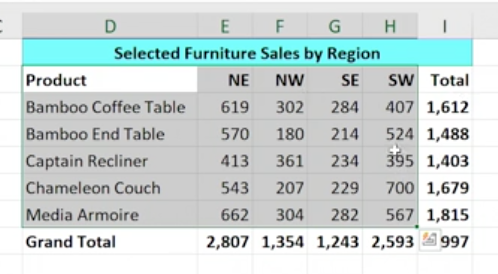
\includegraphics{data.png}
\bigskip \\
\item Alt + F1 is the keystroke shortcut to create a clustered column chart.
\bigskip \\
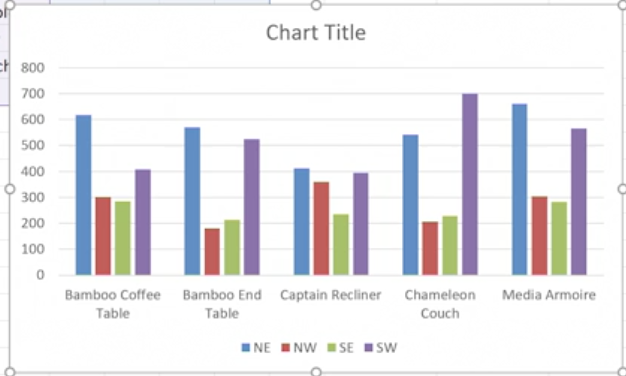
\includegraphics{chart.png}
\bigskip \\
\item To resize the chart while maintaining the same ratio of height to width : while holding the SHIFT key, drag upper-left corner to the required size.
\item Similarly, an Alt + drag causes the boundaries of the chart to match up with the cell boundaries in the background. 
\item To create a chart on a new sheet : Use the key F11.
\item A more standardized method to create charts is by going to Insert -- Recommended Charts.
\item Also, when you highlight data with numbers, a quick analysis button pops up at the bottom right which can also be used to create charts. \\
\bigskip \\
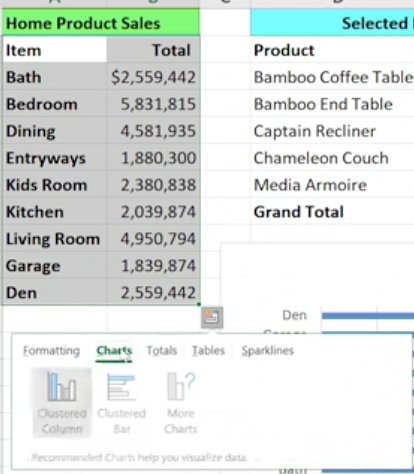
\includegraphics{quick_analysis}
\bigskip \\
\item Remember : The chart is always in-sync with the data! When data changes, so does the chart.
\end{itemize}
\subsection{Exploring Chart types}
\begin{itemize}
\item Under the Design tab in ChartTools : choose the "Switch Row/Columns" option to switch what is represented on the axes of the chart. \\
\bigskip\\
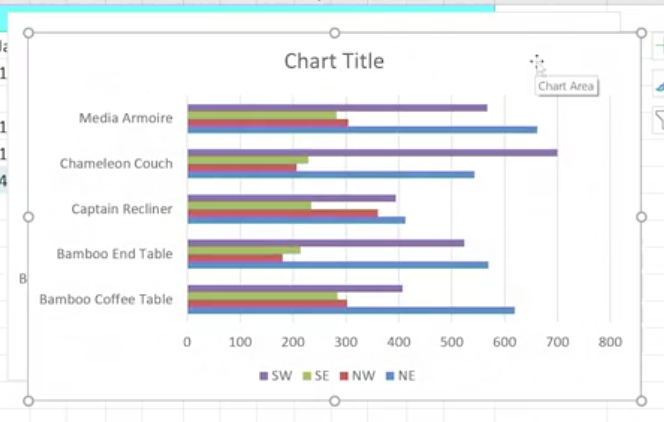
\includegraphics{move_row_1} \\
\bigskip\\
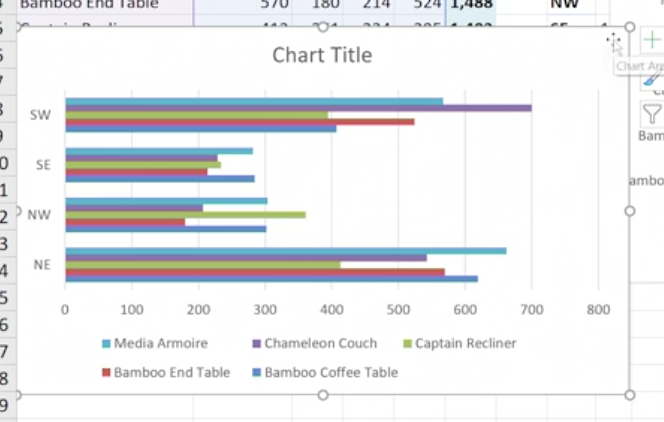
\includegraphics{move_row_2}
\bigskip \\
\item To duplicate a chart use the shortcut Cntrl + D
\item If you are dealing with timeframes (ex. Months) use a Line Chart to represent data.
\item You can change the meaning of a chart by changing the size. Example : The trend may look more incremental.
\end{itemize}
\subsection{Working with Excel Ideas}
\begin{itemize}
\item Ideas is located in the far right of the home tab. Mostly charts and pivot charts are suggested. The aim of this option is to give "ideas" on how me may analyze our data.
\item NOTE : Not all suggestions will be perfect, so be mindful of that!
\end{itemize}
\section{ADJUSTING WORKSHEET VIEWS}
\subsection{Freezing and Unfreezing panes}
\begin{itemize}
\item You can freeze certain rows/columns by going to the tab View -- Freeze Panes.
\item Note : This feature has nothing to do with Printing.
\item useful when you need to freeze first row or/and column, to have context of your data as you scroll through the worksheet,
\item Note : This feature does not work with undo-redo.
\item TIP : To freeze both the first row and column : Click on cell B2 and select the freeze panes option. Everything one row above and to the left gets frozen.
\end{itemize}
\subsection{Splitting screens horizontally and vertically}
\begin{itemize}
\item Using the split function found in the VIEW tab : we can split the sheet vertically or horizontally to simultaneously scroll through two parts of the sheet.
\bigskip\\
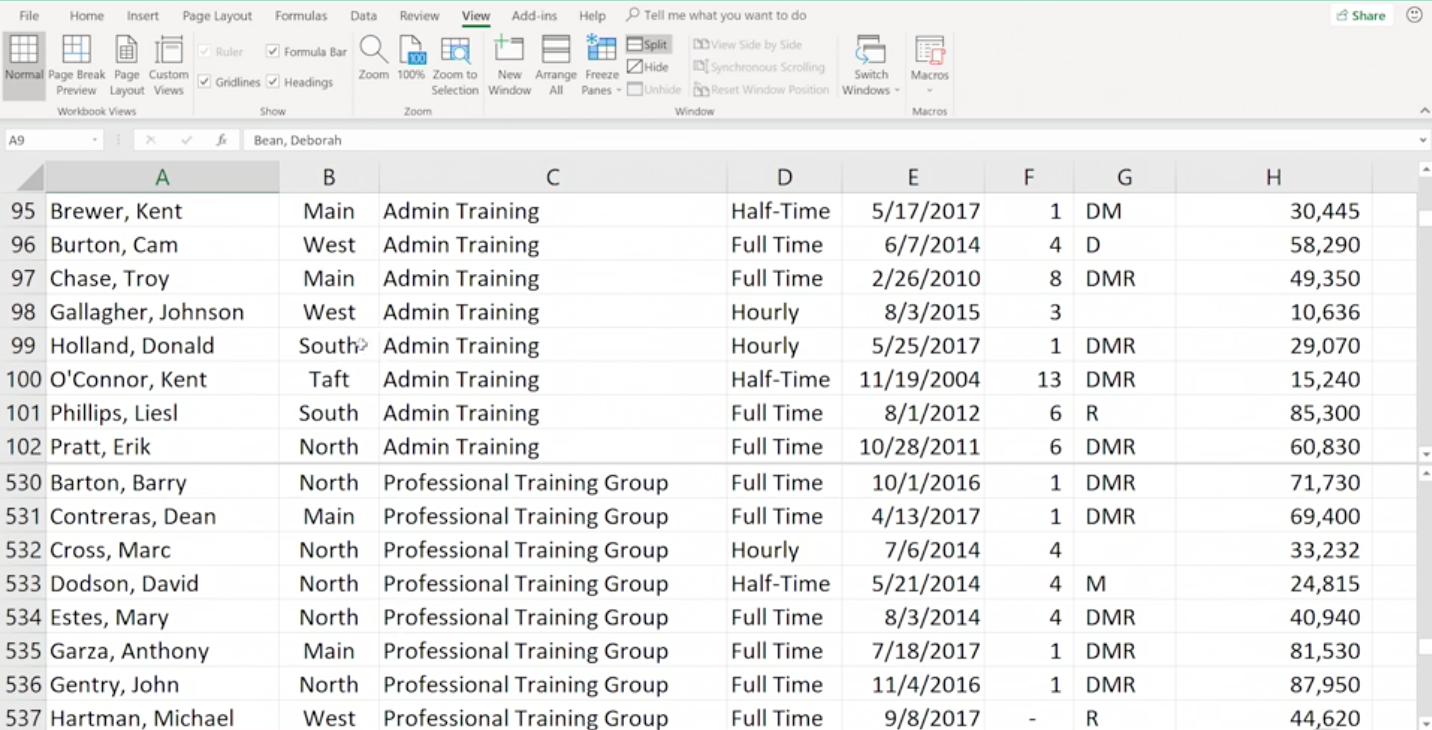
\includegraphics[scale=0.5]{splitScreen}
\bigskip\\
\item To split vertically : Click on the column letter from which you want the split to occur.
\item To exit the split preview : double click on the split line or click on the split feature again.
\item If you click on a cell that is not at the edge of the sheet, Excel gives you a four-way split starting from the selected cell. You are likely to not use this as it is quite confusing. 
\end{itemize}
\end{document}  